\chapter{Pflichtenheft}
\begin{tabular}{ll}
	\hline
	\textbf{Projektbezeichnung:}& \parbox{8cm}{Empfangsstation für globales\\ Satellitenbodenstationsnetzwerk 
		SatNOGS} \\
	\hline
	\textbf{Projektleiter:} & Jakob Metzler \\
	\hline
	\textbf{Erstellt am:} & 25.09.2023 \\
	\hline
	\textbf{Letze Änderung am:} & 07.10.2023 \\
	\hline
	\textbf{Status:}  & Review \\
	\hline
	\textbf{Aktuelle Version: }& 1.2 \\
	\hline
\end{tabular}

\section{Änderungsverslauf}
\begin{tabular}{|c|c|c|c|c|c|c|}
	\hline
	\textbf{Nr.}& \textbf{Datum} & \textbf{Version} & \textbf{\parbox{2cm}{Geänderte\\ Kapitel}} & \textbf{\parbox{1.5cm}{Art der\\ Änderung}} & \textbf{Autor} & \textbf{Status} \\
	\hline
	1 & 25.09.2023 & 1.0 & Alle & Erstellung & \parbox{1.5cm}{Jakob Metzler} & - \\
	\hline
	2 & 02.10.2023 & 1.1 & Alle & Bearbeitung & \parbox{1.5cm}{Jakob Metzler} & Bearbeitung \\
	\hline
	3 & 07.10.2023 & 1.2 & Alle & Korrektur & \parbox{1.5cm}{Jakob Metzler} & Review \\
	\hline
\end{tabular}

\section{Einleitung}
Das vorliegende Pflichtenheft enthält die an die Diplomarbeit gestellten funktionalen sowie nicht
funktionalen Anforderungen. Es dient als Basis für die Ausarbeitung und anschließende schriftliche 
Arbeit und bildet somit einen zentralen Bestandteil der späteren Beurteilung. Alle zuvor zwischen 
Projektmitgliedern und Betreuungslehrer getroffenen Absprachen verlieren in der Regel durch das 
Pflichtenheft ihre Gültigkeit – sofern hier nichts Gegenteiliges vermerkt ist. Mit den Anforderungen 
werden die Rahmenbedingungen für die Entwicklung festgelegt, die von den Projektmitgliedern im 
Pflichtenheft detailliert ausgestaltet werden.

\section{Allgemeines}
\subsection{Ziel und Zweck des Dokuments}
Dieses Pflichtenheft beschreibt die Vorgaben für funktionale sowie nicht-funktionale Anforderungen 
an die Diplomarbeit „Empfangsstation für globales Satellitenkommunikationsnetzwerk SatNOGS“. 

\subsection{Ausgangssituation}
Im Rahmen der Ausbildung an der Höheren Technsichen Bundeslehr- und Versuchsanstalt Rankweil 
wird zur erfolgreichen Reife- und Diplomprüfung eine Diplomarbeit erstellt, dessen Anforderungen in 
diesem Dokument beschrieben werden. 

\subsection{Projektbezug}
Das vorliegende Projekt ist ein unabhängiges Projekt welches ohne zusammenhängende Verpflichtung 
in Bezug, auf den im Jahr 2024 von Technischen Universität Wien in den Low-Earth-Orbit beförderten 
Satelliten STS1 entsteht. 

\subsection{Abkürzungen}
\begin{tabular}{ll}
	\hline
	LEO: & Low-Earth-Orbit \\
	\hline
	AHS: & Allgemeinbildende Höhere Schule \\
	\hline
	BHS: & Berufsbildende Höhere Schule \\
	\hline
	DA: & Diplomarbeit \\
	\hline
\end{tabular}

\subsection{Teams und Schnittstellen}
Hauptverantwortliche dieses Projekts sind Projektleiter und Projektmitglieder, in deren 
Verantwortung die Umsetzung und Ausarbeitung des Projekts fällt. Unterstützt wird das Projektteam 
bei technischen und/oder formalen Unklarheiten durch den Betreuer, welcher anschließend auch 
maßgeblich an der Beurteilung des Projekts beteiligt ist.

\begin{tabular}{|c|c|c|c|}
	\hline
	Rolle(n) & Name & E-Mail & Tätigkeit \\
	\hline
	Projektleiter & Jakob Metzler & jakob.metzler@student.htl-rankweil.at & \parbox{2cm}{Organisation,\\ Hardware, Software}\\
	\hline
	Projektmitglied & Gabriel Ritter & gabriel.ritter@student.htl-rankweil.at & Hardware, Software \\
	\hline
	Betreuer & Christian König & christian.könig@htl-rankweil.at & Betreuung der DA \\
	\hline
\end{tabular}

\section{Konzept}
\subsection{Ziel der Anbieter}
Das Ziel der Anbieter, welche in diesem Fall die Projektmitglieder darstellen, ist es, durch die Abgabe 
einer ausgereiften schriftlichen Dokumentation sowie eines funktionierenden Endprodukts eine 
positive und möglichst gute Bewertung für die Diplomarbeit zu erhalten.

\subsection{Ziel und Nutzen des Anwenders}
Der Anwender wird folglich in zwei Gruppen aufgeteilt, welche unterschiedliche Ziele verfolgen oder 
Nutzen aus der Diplomarbeit ziehen.\\

\underline{Anwender in Bezug auf die Diplomarbeit:}\\
Das Ziel des Anwenders in Bezug auf die Diplomarbeit besteht darin, eine vollständige Diplomarbeit zu 
erhalten, um diese anschließend basierend auf der Erfüllung Ihrer funktionalen als auch nicht
funktionalen Anforderung bewerten zu können. \\
\underline{Anwender in Bezug auf das im Rahmen der Diplomarbeit entstehende Produkt:}\\ 
Ziel der Anwender in Bezug auf das im Rahmen der Diplomarbeit entstehende Produkt ist es, eine 
vollständig funktionstüchtige Plattform zu erhalten, welche es ermöglicht, die Daten von Satelliten im 
LEO zu empfangen und darzustellen, um diese anschließend für Analysen oder Interpretationen zu 
verwenden.

\subsection{Zielgruppen}
Auch die Zielgruppen können, wie die Anwender in zwei Gruppen aufgeteilt werden.\\

\underline{Zielgruppe in Bezug auf die Diplomarbeit: }\\
Bei der Zielgruppe in Bezug auf die Diplomarbeit handelt es sich um fachkundige Personen. Das 
Ergebnis und die Dokumentation der Diplomarbeit sollen aus diesem Grund nicht zu abstrakt 
dargestellt werden, sondern technisch detailliert und qualitativ hochwertig ausgeführt sein.\\

\underline{Zielgruppe in Bezug auf das im Rahmen der Diplomarbeit entstehende Produkt: }\\
Die Zielgruppe in Bezug auf das im Rahmen der Diplomarbeit entstehende Produkt besteht aus 
Schülern und Lehrpersonen aus AHS und BHS. Es muss also von verschiedenen Wissensstandpunkten 
im Gebiet der Telekommunikation, Informatik und Elektronik ausgegangen werden und dennoch eine 
für jede spezifische Zielgruppe zumutbare Bedienfreundlichkeit sichergestellt werden. Erforderlich 
sind aus diesem Grund zum Beispiel Erklärungen oder Hinweise für beispielsweise einstellbare 
Parameter. 

\section{Funktionale Anforderungen}
\subsection{Empfangen von Telekommunikationsdaten}
Hauptanforderung und Ausgangspunkt aller weiteren funktionalen Anforderungen ist der 
kontinuierliche Empfang von Daten im 430MHz/70cm-Band eines Satelliten, welcher sich im LEO 
befindet.\\

\subsection{Decodieren und Zuordnen empfangener Daten}
Die empfangenen Daten sollen decodiert und zugeordnet werden. Dabei ist unter Decodieren, das 
basierend auf dem Protokoll, welches zur Übertragung verwendet wurde, Trennen der Nutzdaten von 
anderen Datenframes, Headern oder Prüfsummen zu verstehen. Unter zuordnen ist zu verstehen, wie 
die verschiedenen Daten ihrer Bedeutung zugeordnet werden. Zum Beispiel werden die Nutzdaten von 
Datenpaket D1 der Temperatur an Fühler F1 zum Zeitpunkt T1 zugeordnet, also beschrieben, auf was 
sich die Daten im Paket beziehen.\\

\subsection{Grafische Darstellung empfangener Daten}
Die empfangenen Daten sollen zur leichteren Interpretation und Analyse grafisch sinnvoll und übersichtlich dargestellt werden. Es soll dadurch ermöglicht werden, Zusammenhänge zu visualisieren oder zeitliche Verläufe darzustellen.\\

\section{Nichtfunktionale Anforderungen}
\subsection{Allgemeine Anforderungen}
Das herzustellende Produkt sollte so gestaltet sein, dass es den für die Region (Mitteleuropa) typischen 
Belastungen durch UV-Strahlung, Regen, Schnee, Hagel und Sturm standhält.\\ 

\subsection{Dokumentative Anforderungen}
Um für die Bewertung der Diplomarbeit eine Grundlage zu bieten, wird eine ausführliche 
Dokumentation vorausgesetzt. Diese soll sowohl theoretische Erklärungen über die Themen, welche 
in der Durchführung behandelt werden, beinhalten, als auch eine technische Dokumentation über die 
Durchführung selbst.\\

\subsection{Technische Anforderungen}
Das herzustellende Produkt soll mit europäischer Netzspannung betrieben werden können. (230 V 
± 23 V / 50 Hz ± 0,2 Hz)\\

\section{Rahmenbedingungen}
Folglich werden die Rahmenbedingungen für die Durchführung der bisher beschriebenen 
Arbeit festgelegt.\\

\subsection{Zeitplan}
Die Abgabe der Diplomarbeit hat spätestens am 3. April 2024 zu erfolgen. Um dieses Ziel zu 
erreichen, soll die gesamte Hardware spätestens am 5. Februar 2024 fertiggestellt werden und bis 
zum 19. März 2024 eine Erstfassung der schriftlichen Diplomarbeit zu Korrektur erstellt werden. Für 
jedes Teammitglied wird hierfür eine Arbeitszeit von jeweils 180 Stunden eingeplant.\\

\subsubsection{Meilensteinplan}

\begin{enumerate}
	\item 12.05.2023 - \textbf{Themenfindung}\\
	\underline{Ergebnis:} Die erfolgreiche Besprechung mit dem Betreuer ergibt den Startschuss für die 
	Diplomarbeit.
	
	\item 28.09.2023 - \textbf{Kickoff}
	\underline{Ergebnis: }Die erfolgreiche Besprechung mit dem Betreuer ergibt den Startschuss für die 
	Diplomarbeit.
	
	\item 29.09.2023 - \textbf{Antrag eingereicht}\\
	\underline{Ergebnis: }Der Diplomarbeitsantrag wurde eingereicht.
	
	\item 16.10.2023 - \textbf{Pflichtenheft erstellt}\\
	\underline{Ergebnis: }Das Pflichtenheft wurde beim Betreuer abgegeben 
	
	\item 16.10.2023 - \textbf{Kooperationspartner gefunden}\\
	\underline{Ergebnis: }Ein Unternehmen hat sich bereit erklärt als Partner in der Diplomarbeit zu fungieren. 
	
	\item 23.10.2023 - \textbf{Antennentyp bestimmt}\\
	\underline{Ergebnis: }Der im Rahmen der Diplomarbeit zu bauende Antennentyp ist festgelegt. 
	
	\item 01.12.2023 - \textbf{Antenne fertiggestellt}\\
	\underline{Ergebnis: }Die im Rahmen der Diplomarbeit zu bauende Antenne wurde fertigstellt.
	
	\item 11.12.2023 - \textbf{Empfangsmodul fertiggestellt}\\
	\underline{Ergebnis: }Eine finale Empfangsmodul-Hardware liegt vor. 
	
	\item 15.01.2024 - \textbf{Übersetzung und Zuordnung der empfangenen Daten}\\
	\underline{Ergebnis: }Back-End Empfangssoftware ist funktionstüchtig und übersetzt und ordnet die 
	empfangenen Daten ordnungsgemäß zu.
	
	\item 29.01.2024 - \textbf{Visualisierung der empfangenen Daten}\\
	\underline{Ergebnis: }Eine Visualisierung der empfangenen Daten ist möglich. 
	
	\item 30.01.2024 - \textbf{Eigenschaften der Antennen aufgenommen}\\
	\underline{Ergebnis: }Eigenschaften verschiedener Antennen wurden in einer Messzelle aufgenommen. 
	
	\item 05.02.2024 - \textbf{Empfangsstation fertiggestellt}\\
	\underline{Ergebnis: } Die Daten werden über die Antenne empfangen und anschließend übersetzt und 
	zugeordnet, um sie schließlich grafisch übersichtlich darzustellen.
	
	\item 19.03.2024 - \textbf{Erstfassung der schriftlichen Dokumentation}\\
	\underline{Ergebnis: } Alle Themen wurden in der schriftlichen Diplomarbeit ausgearbeitet und zum 
	Korrekturlesen an geeignete Personen weitergeleitet. Der Inhalt kann vom Betreuer geprüft und 
	ggf. noch leicht abgeändert werden.
	
	\item 03.04.2024 - \textbf{Abgabe der schriftlichen Diplomarbeit}\\
	\underline{Ergebnis: } Die schriftliche Diplomarbeit wurde abgegeben. 
\end{enumerate}

\subsection{Technische Anforderungen}
Für die Umsetzung der Diplomarbeit ist folgendes Hard- \& Softwaremäßiges Equipment notwendig:
\begin{enumerate}
	\item Netzwerkanalysator
	\item Oszilloskop
	\item SolidWorks
	\item Messzelle mit dementsprechendem Equipment
	\item Equipment aus dem Hochfrequenzlabor
	\item standardmäßig eingerichtete Elektronikwerkstatt (Lötkolben, Multimeter, Zangen, etc...)
\end{enumerate}

\subsection{Problemanalyse}
In den nächsten Punkten werden mögliche Probleme und deren Gegenmaßnahmen beschrieben.  

\subsubsection{Lieferverzögerungen}
Viele für die Diplomarbeit notwendige Bauteile und Komponenten können nicht lokal erworben 
werden und bedürfen einer Lieferung von speziellen Händlern. Werden Lieferketten unterbrochen 
oder verzögert, verschiebt das den gesamten Zeitplan der Diplomarbeit nach hinten, was die 
schlussendliche Abgabe gefährden könnte. Aus diesem Grund sind kritische Bauteile und 
Komponenten früh genug zu bestellen und deren Lieferstatus zu beobachten. Kommt es dennoch zu 
Verzögerungen oder Lieferstopps, muss schnellstmögliche eine Alternative für das Bauteil oder die 
Komponente gefunden und bestellt werden, was nicht zuletzt zu höheren Gesamtkosten des Projekts 
führen kann.

\subsubsection{Mangel an Know-How}
Können die Ursachen auftretender Probleme nicht identifiziert werden, liegt das meistens an 
mangelndem Know-how. In diesem Fall sind Personen, welche im betroffenen Bereich bereits viel 
Erfahrung haben, ausfindig zu machen und um Hilfe oder Ratschläge zu bitten. 

\subsubsection{Kein Zugang zu einer Messzelle}
Für die qualitative Charakterisierung einer Antenne und die Aufnahme weitere Eigenschaften wird eine 
professionelle Messzelle benötigt. Kann kein Unternehmen gefunden werden, welches Interesse an 
einer Kooperation hat und seine Messzelle zur Verfügung stellt, muss mit vorhandenen Geräten 
versucht werden, eine möglichst genaue Charakterisierung durchzuführen. Hierbei sind 
selbstverständlich enorme Qualitätseinbußen in Kauf zu nehmen. 

\subsection{Qualität}
Es wird eine den zur Verfügung stehenden Werkzeugen zumutbare qualitative Verarbeitung für das zu 
entstehende Produkt im Rahmen der Diplomarbeit vorausgesetzt. Mögliche im Projekt programmierte 
Software hat eine einheitliche Naming-Convention zu verwenden und in Bezug auf die Funktion 
dokumentiert sowie kommentiert zu sein. Der schriftliche Teil der Diplomarbeit hat mit besten Wissen 
und Gewissen auf Rechtschreib- sowie Flüchtigkeits- und Tippfehler überprüft und korrigiert zu sein.

\section{Abgabebedingungen}
Das Projekt gilt ab Übergabe der schriftlichen Diplomarbeit von den Projektmitgliedern an die 
zuständige Stelle am 03. April 2024 als abgegeben. Die Abgabe hat sowohl in digitaler als auch in 
zweifach ausgeführter gebundener Version zu erfolgen. 

\section{Anhang}
Auf den nachfolgenden Seiten ist der Diplomarbeitsantrag zu finden, welcher ebenfalls als Teil dieses 
Pflichtenhefts sowohl funktionale als auch nicht-funktionale Anforderungen enthält.
\newpage

07.10.23, 23:33

{\huge Empfangsstation für globales Satellitenbodenstationsnetzwerk SatNOGS}

\begin{tabular}{|c|}
	\hline
	Verlauf \\
	\hline
	\parbox{\textwidth}{28.09.2023 um 10:01 Die Themenstellung $"$Empfangsstation für\\ globales Satellitenbodenstationsnetzwerk \\SatNOGS$"$ (Gabriel RITTER, Jakob METZLER) wurde eingereicht.}
	 \\
	\hline
	\parbox{\textwidth}{19.09.2023 um 10:09 Die Themenstellung $"$Empfangsstation für globales Satellitenbodenstationsnetzwerk SatNOGS$"$ (Jakob METZLER) wurde vom Betreuer/von der Betreuerin akzeptiert.} \\
	\hline
\end{tabular}

{\large Schule\\}
Höhere technische Bundeslehr- und Versuchsanstalt RANKWEIL

{\large Abteilung(en)\\}
Hauptverantwortlich: Elektronik und Technische Informatik

{\large AV\\}
Hauptverantwortlich: Leopold MOOSBRUGGER

{\large Abschließende Prüfung\\}
2024

{\large Betreuer/innen\\}
Hauptverantwortlich: Christian KÖNIG (C)

{\large Ausgangslage}
Im Jahr 2024 befördert das SpaceTeam der Technischen Universität Wien ihren neuesten Satelliten STS1 in den nicht geostationären Low-Earth-Orbit. Die vom Satelliten gesendeten Sensordaten werden durch die Empfangsstation ausgewertet und anschließend auf einer grafischen Benutzeroberfläche in Echtzeit dargestellt.

{\large Projektteam (Arbeitsaufwand)}

\begin{tabular}{|c|c|c|c|}
	\hline
	\textbf{Name} & \textbf{Individuelle Themenstellung} & \textbf{Klasse} & \textbf{Arbeitsaufwand} \\
	\hline
	\parbox{4cm}{Jakob METZLER (Hauptverantwortlich)} & \parbox{5cm}{ Gruppenleitertätigkeit, Recherche, Entwicklung der Antenne, Aufbau der Hardware, Charakterisierung der Antenne, Software (Frontend)} & 5AHEL & 180 Stunden\\
	\hline
	Gabriel RITTER & \parbox{5cm}{Recherche, Entwicklung der Antenne, Aufbau der Hardware, Charakterisierung der Antenne, Software (Backend)} & 5AHEL & 180 Stunden\\
	\hline
\end{tabular}

\begin{figure}
	\centering
	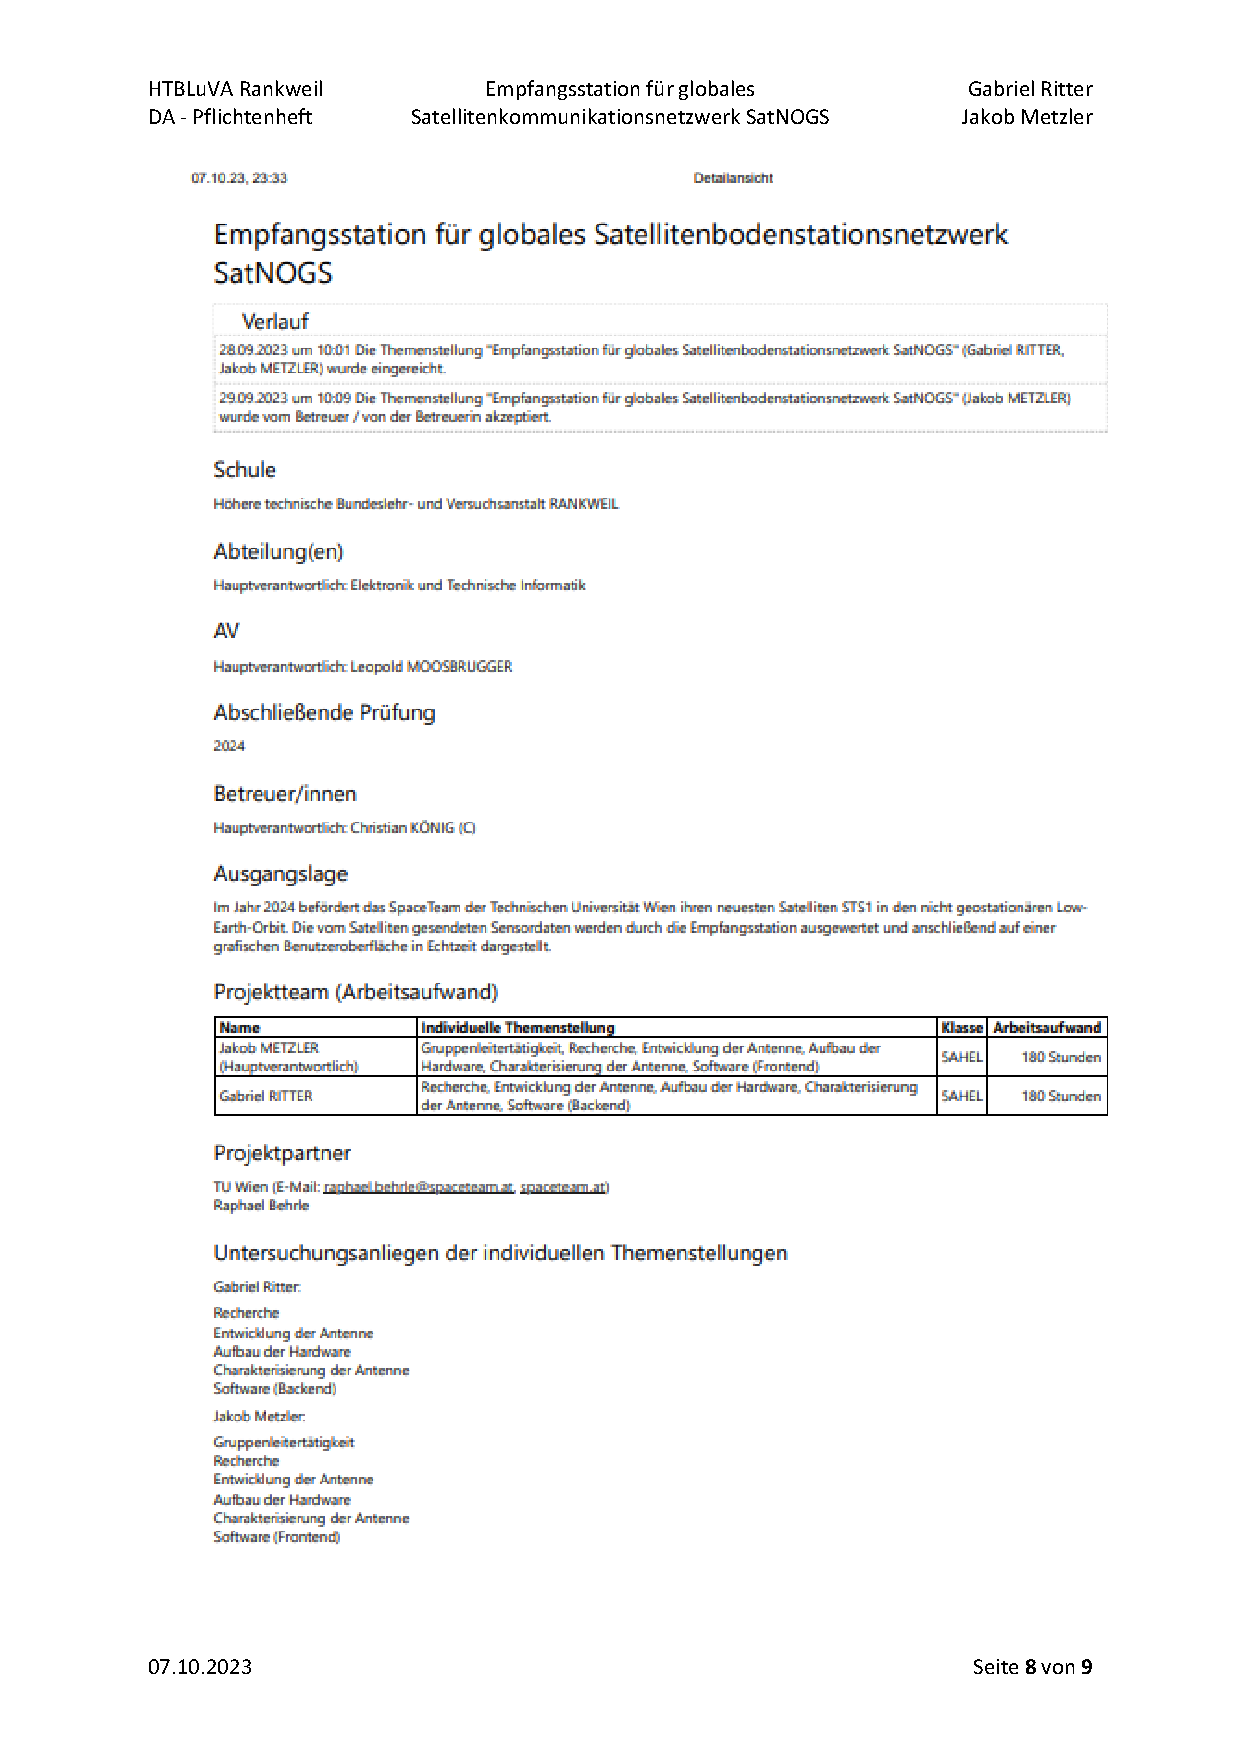
\includegraphics[width=\textwidth]{../ref/DA_Metzler_Ritter_Pflichtenheft_v1.2-page8.pdf}
\end{figure}

\begin{figure}
	\centering
	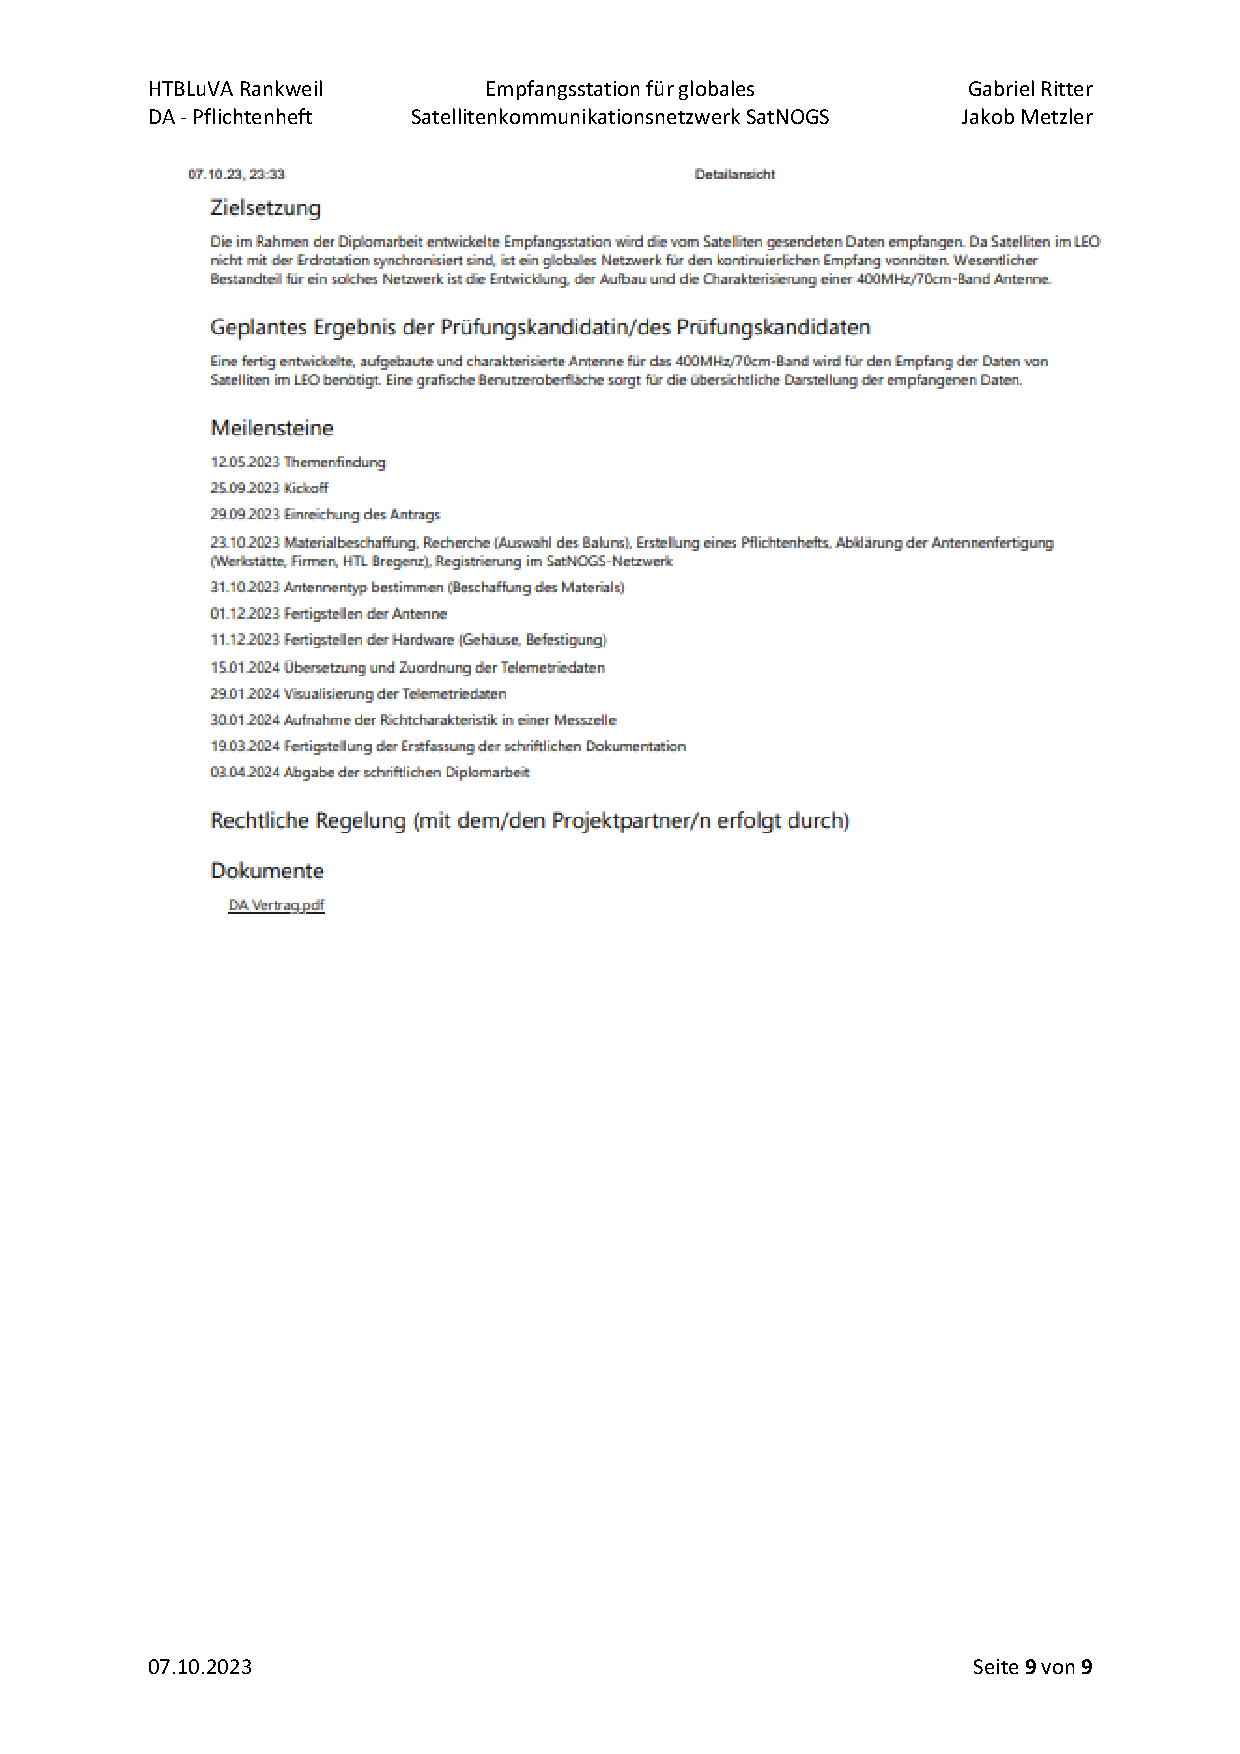
\includegraphics[width=\textwidth]{../ref/DA_Metzler_Ritter_Pflichtenheft_v1.2.-page9pdf.pdf}
\end{figure}


\pagebreak
